\documentclass[11pt]{article}
\setlength{\parindent}{0em}
\setlength{\parskip}{1em}
\usepackage{titlesec}
\usepackage{graphicx}
\usepackage{pgfplots}
\usepackage{subcaption}
\usepackage{float}
\pgfplotsset{width=\textwidth,compat = 1.17}
\usepackage{tikzscale}
\usepackage{blindtext}
\usepackage{multicol}
\usepackage[inline]{enumitem}
\usepackage{booktabs,caption}
\usepackage{natbib}
\bibliographystyle{apa}
\usepackage[flushleft]{threeparttable}
\usepackage[font=small]{caption}
\providecommand{\keywords}[1]{\textbf{\textit{Keywords ---}} #1}
\usepackage[
separate-uncertainty = true,
multi-part-units = repeat
]{siunitx}
\usepackage{hyperref}
% Data
\graphicspath{ {D:\/SciWriting} }
\begin{filecontents*}{data.csv}
	a,b,c,d,e,f
	0,67.4,68.6,68.8,68.6,68.6
	1,66.9,35.3,46.1,25.4,55.1
	2,66.1,23.2,29.3,20.3,44.4
	3,65.5,20,20.9,20.1,32.1
	4,64.5,20.1,20.1,20,23.5
	5,63.9,19.8,20.2,20,20.1
	6,63,19.9,19.9,19.9,19.8
	7,62,20.2,20.2,20.1,19.9
\end{filecontents*}
% Title Page
\title{\Huge Comparison of Coffee Containers based on Temperature Preservation Capabilities}
\author
{
	\href{anhky.nguyen@student.kuleuven.be}{Anh Ky Nguyen} \\ 
	Electronics Engineering \\ 
	Faculty of Engineering Technology, Campus Group T, Leuven \\ 
	Vesaliusstraat 13, 3000 Leuven, Belgium \\ 
	anhky.nguyen@student.kuleuven.be \\ \\
	Supervisor: \href{eva.cordery@kuleuven.be}{Eva Cordery}	\\
	Faculty of Engineering Technology, Campus Group T, Leuven \\ 
	Vesaliusstraat 13, 3000 Leuven, Belgium \\ 
	eva.cordery@kuleuven.be 	
}
\date{}

\begin{document}
\maketitle
\titlespacing\section{0pt}{10pt plus 2pt minus 2pt}{0pt plus 2pt minus 2pt}
\titlespacing\subsection{0pt}{10pt plus 2pt minus 2pt}{0pt plus 2pt minus 2pt}
\titlespacing\subsubsection{0pt}{10pt plus 2pt minus 2pt}{-5pt plus 2pt minus 2pt}
\titleformat{\section}[block]{\color{black}\huge\bfseries\filcenter}{}{1em}{}
\titleformat{\subsubsection}{}{\thesubsubsection}{1em}{\itshape}
\begin{keywords}
	Thermal conductivity, coffee, drink containers, heat preservation, insulation materials
\end{keywords}

%----------------------------------------------------------------
\begin{abstract}
	
As coffee becomes the norm for many citizens, the need for a practical container that can keep coffee at the ideal temperature range (50 – 70°C) for an extended duration ($\geq$ 6 hours) prevails. This paper investigated the heat preservation efficacy of different drink containers and whether it improves by pre-treating them using hot water. The empirical data illustrated a negative correlation between the total heat loss and the thermal conductivity of materials used for the containers. Evidence from the experiment also confirmed that brewed coffee stored in the preheated container had a higher average temperature than its unrinsed counterpart. The study suggested that general consumers choose vacuum flasks and rinse them before storing any hot beverages for the best results.

\end{abstract}

\pagebreak
%----------------------------------------------------------------
\section*{Introduction}

World coffee consumption has achieved an average growth of 2.7$\%$ over the last five years \cite{InternationalCoffeeOrganizationICO2019}. Consumers have become more knowledgeable and demanding regarding the quality and preservation of coffee. As such, beverage containers have grown into a debatable topic among avid drinkers. The main arguments focus on the heat preservation capabilities of the canisters since the serving temperature of coffee plays a vital role in its taste.

Ingesting too hot coffee heightens the risk of scald burns while a colder drink may not satiate the drinker. The preferred drinking temperature of coffee is found to be $\SI{60 \pm 8.3}{\celsius}$ \citep{Brown2008}. The reason is that coffee exhibits different flavour notes depending on the serving temperature \citep{PMID:27765259}. On the other hand, reheating cold coffee is not advocated since it will bolster the amount of caffeine and chlorogenic acid (CGA) – two compounds responsible the level of astringency in coffee – to an unwanted level for the consumer \citep{Niseteo2012}. Thus, the best strategy is to keep the freshly brewed coffee at the favourable temperature region (\SI{52}{\celsius} – \SI{68}{\celsius}) as long as possible before serving.

On the market, there are many kinds of containers varying in construction and materials. Thermoplastic (plastic with unchanged properties even after multiple mouldings) is often used in drink containers due to their low-cost and lightweight nature. Two notable resin types for food packaging are Polypropylene (PP) and Polystyrene (PS), which accounts for almost one-fourth of plastic demand in Europe \citep{PlasticsEuropetheAssociationofPlasticsManufacturersinEurope2019}. On the other hand, glass bottles attract consumers because they are environmentally superior to plastic and metal canisters \citep{InSitesSurvey2018}. With their inert attributes, glass containers will hardly contaminate their contents after heavy use. 


\begin{figure}[h!]
	\centering
	\caption{A cut-away drawing describing components of a thermos bottle. \citep{SamuelJ.LingWilliamMoebs2016}}
	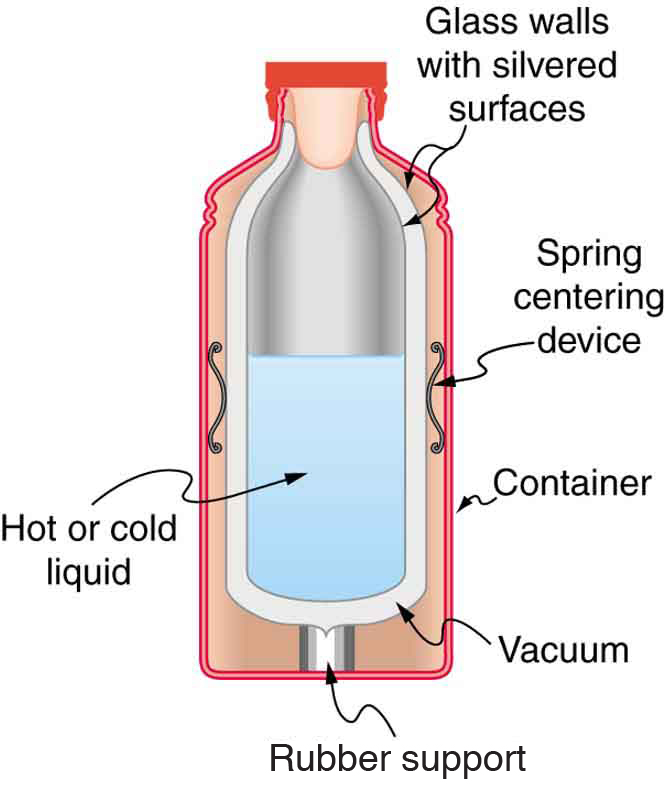
\includegraphics[width=0.5\textwidth,height=0.375\textheight]{Tdiagram}
	\label{Figure 1}
\end{figure}

\pagebreak

Situating at a higher price point are thermos flasks (vacuum flasks) built with an outer metal case and an inner double-walled vacuum chamber (\autoref{Figure 1}). The empty area between layers prevents heat transfer from the content to the environment through conduction and convection. A silver coating is applied on the glass walls to reduce the effect of thermal radiation. Additionally, rinsing the vacuum flasks with hot water is prevalent among drinkers. The hypothesis is that preheating the container will improve its heat insulation.

\begin{table}[h!]
	\centering
	\begin{threeparttable}
		\caption{Thermal conductivity of some materials often used for drink containers. The vacuum itself is not a material, but its mechanics are employed in the thermos flasks.}
		\label{Table 1}
		\begin{tabular*}{\textwidth}{ @{\extracolsep{\fill}} cc}
			\toprule
			Material & Thermal conductivity (\SI{}{W/m.K}) \\
			\midrule 
			Glass \textsuperscript{1} 				  & 0.67    \\
			Stainless steel \textsuperscript{1}  	  & 0.02    \\
			Polystyrene \textsuperscript{1}  			  & 0.15    \\
			Polypropylene \textsuperscript{2}   	  & 1.00    \\
			Vacuum    				  & $\simeq$ 0.00	\\
			\bottomrule
		\end{tabular*}
		\begin{tablenotes}
			\footnotesize
			\centering
			\item \textsuperscript{1} \citep{Young1992}; \textsuperscript{2} \citep{Patti2020}
		\end{tablenotes}
	\end{threeparttable}
\end{table} 

There are three ways that heat can transfer in a bottle: conduction, convection and radiation. Conduction is the process in which thermal energy transfers through collisions of microscopic particles in a solid or liquid body. It has been proven that thermal conductivity values vary substantially between material (\autoref{Table 1}). In addition, convection is the heat generated from molecules in fluid when they become less dense and rise. Radiation is the method of thermal transmission using electromagnetic waves from the heat sources.  

This paper will investigate the thermal preservation efficacy of different coffee containers and how pre-treating the vacuum flask with hot water will improve its heat insulation using empirical data from an experiment. The test subjects include a PP bottle, thermos flasks, a PS cup, a glass bottle and a stainless steel bottle (\autoref{Figure 3}). 
%---------------------------------------------------------------------------------
\section*{Experiment}

\subsection*{Apparatus}

The preparation of coffee involved using a "Phin" metal filter (\autoref{Vfilter}).  To ensure homogenous sampling in the experiment,  only a single type of ground coffee was prepared. Four tablespoons of powder (estimated to be 60g in total) were dropped into the chamber, which was then swayed lightly and put on the spanner. After that, the filter press was applied to flatten the coffee powder surface. Finally, boiling water was poured into the filter chamber so that the coffee juice could be extracted. 

\begin{figure}[H]
	\centering
	\subcaptionbox{"Phin" coffee filter with parts \label{Vfilter}}
		{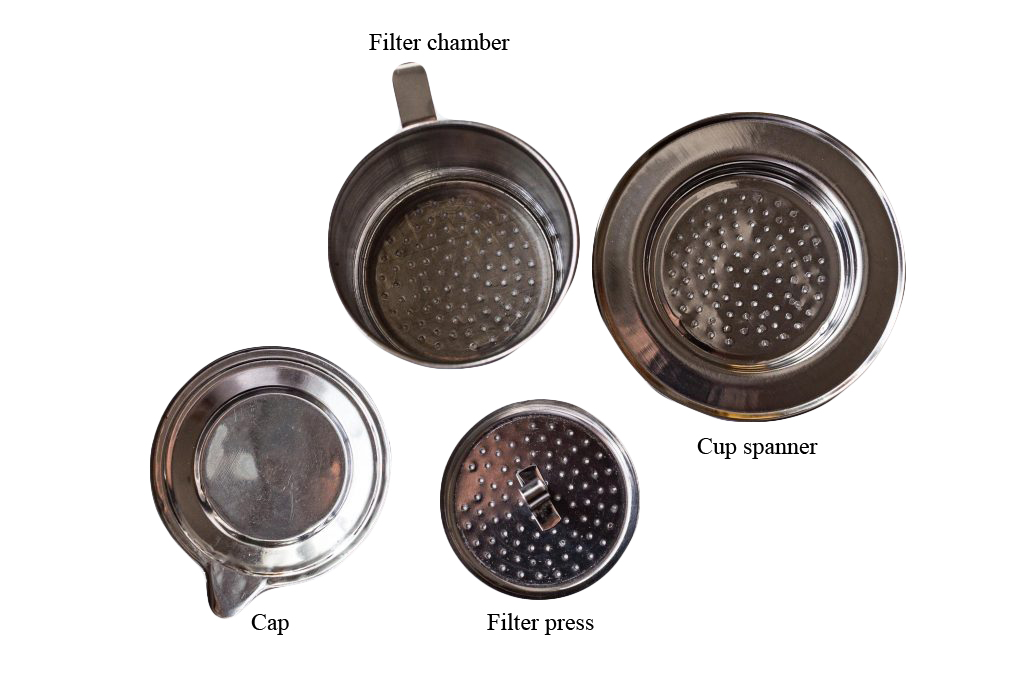
\includegraphics[width=0.8\textwidth,height=0.35\textheight]{Vfilter}}
	\subcaptionbox{Measuring cup \label{Mcup} [\citenum{Norpro2020}]}
		{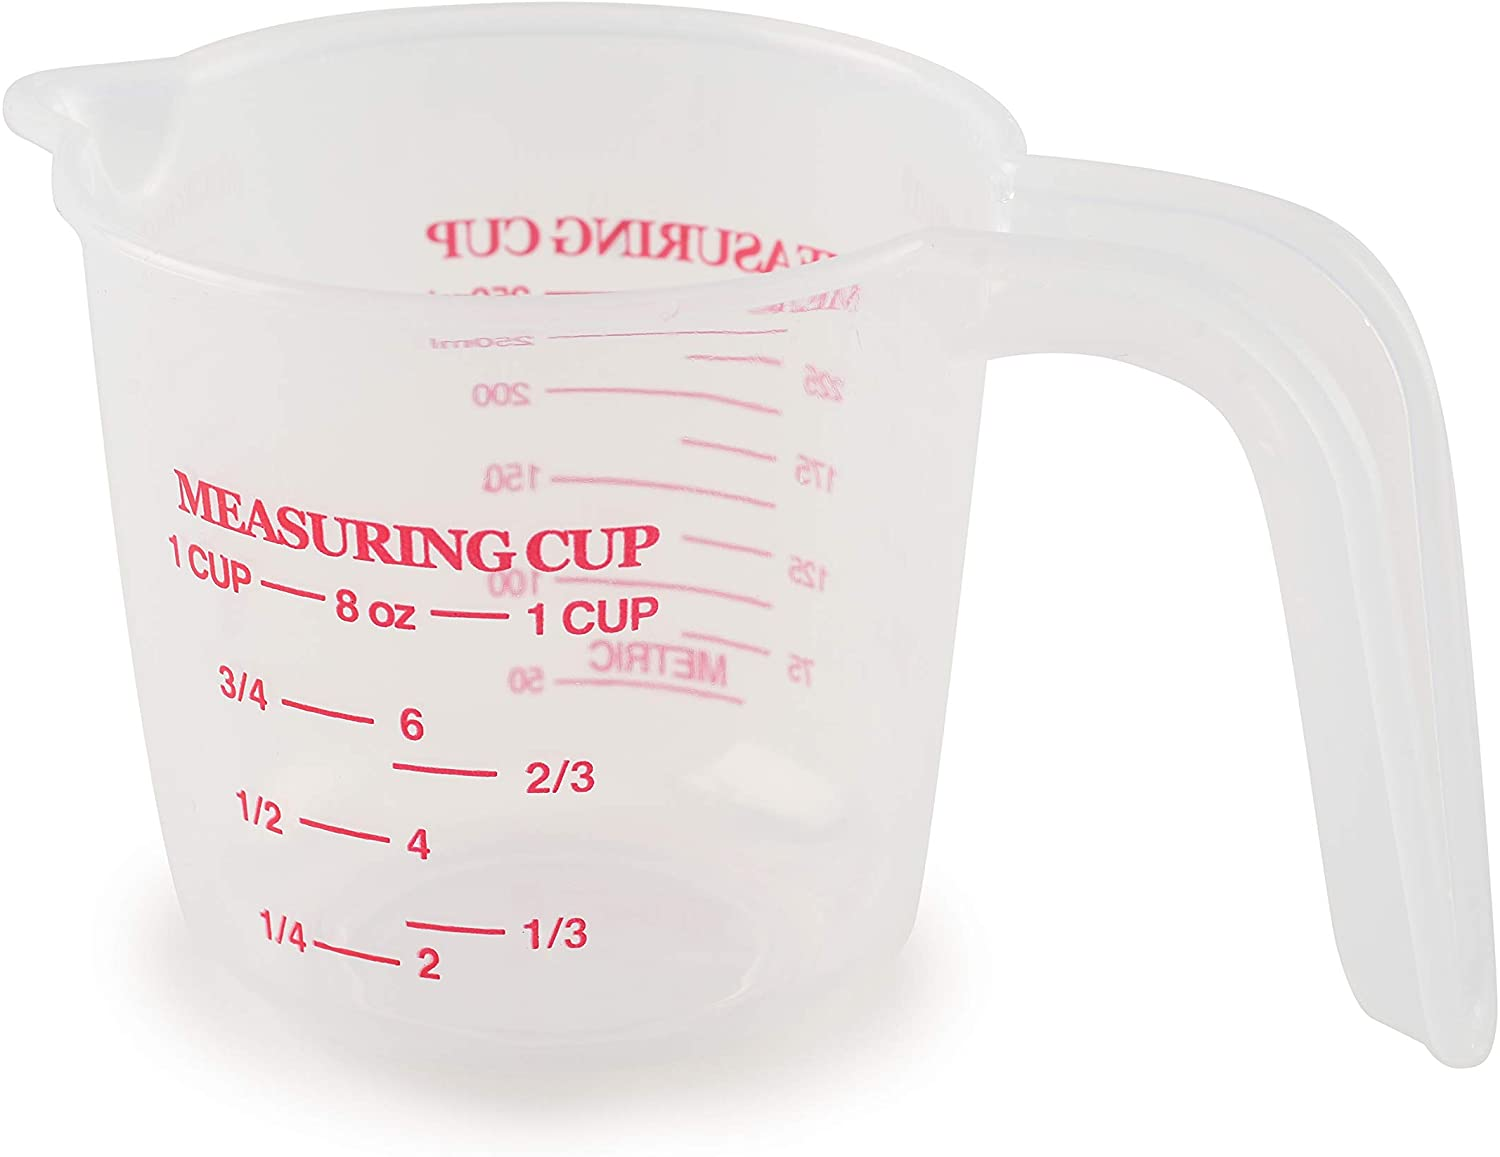
\includegraphics[width=0.3\textwidth,height=0.2\textheight]{Mcup}}
	\subcaptionbox{Thermometer \label{Thermometer} [\citenum{DeltaTrak2020}]}
		{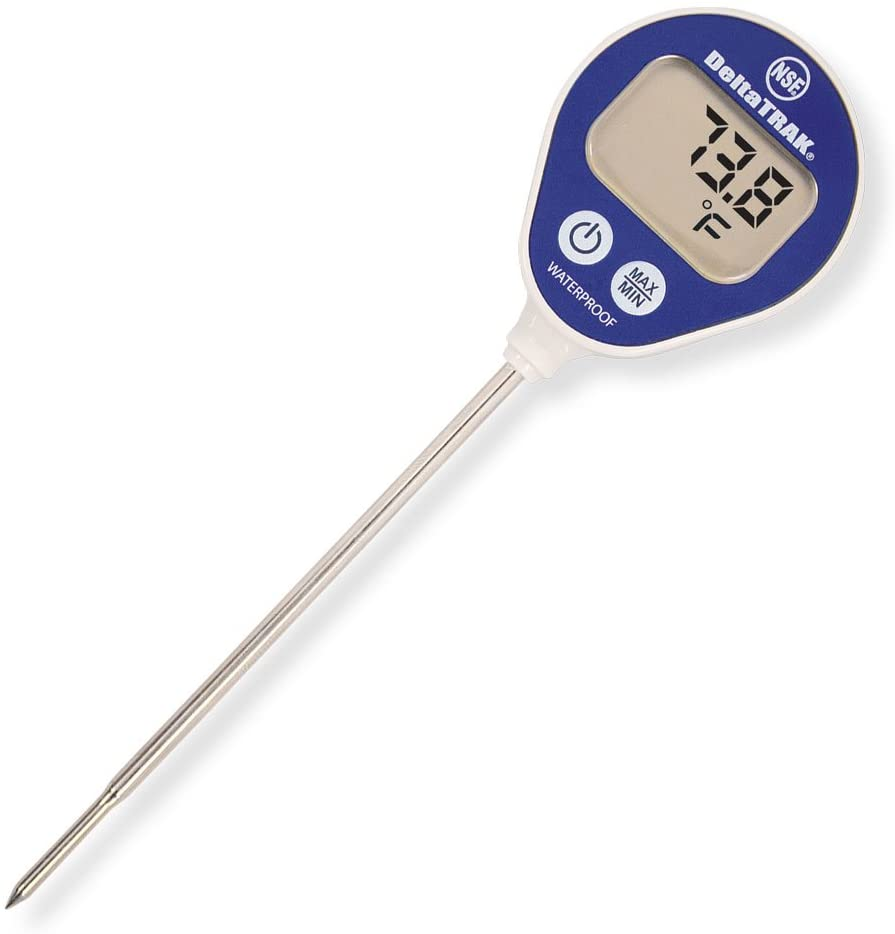
\includegraphics[width=0.3\textwidth,height=0.2\textheight]{Thermometer}}
	\caption{Equipment used in the experiment. The "Phin" filter is for the preparation of coffee. A measuring cup and a thermometer are utilized to check the volume and temperature of all substances in the experiment.}
	\label{Figure 2}
\end{figure}

\pagebreak

The temperature of the substances was checked using a digital food-grade thermometer (\autoref{Thermometer}) with the range from -40 °C to 155 °C (±1$\%$). A measuring cup (\autoref{Mcup}) was included to transfer or measure the quantity of liquid in the experiment. Its capacity was 250 ml while the smallest unit on the gradation was 25 ml. Before the experiment, both tools were cleaned with water and left to dry. The thermometer was also calibrated to ensure accuracy. 

\subsection*{Test subjects}

\bigskip

\begin{figure}[H]
	\centering
	\subcaptionbox{PS cup \label{Styro} [\citenum{RocketIndustrial}]}
	{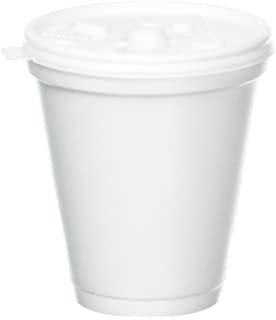
\includegraphics[width=0.3\textwidth,height=0.2\textheight]{Styro}}
	\subcaptionbox{PP bottle \label{pp} [\citenum{IndiaMART}]}
	{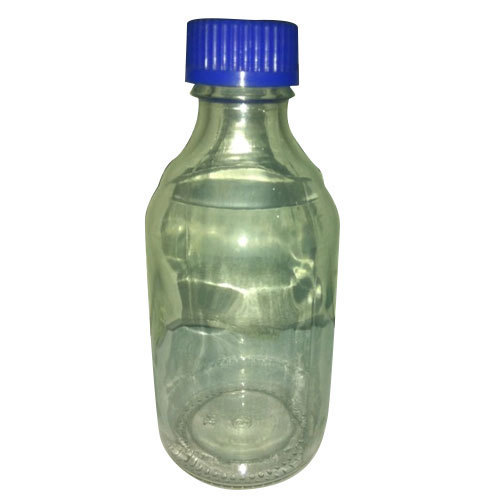
\includegraphics[width=0.3\textwidth,height=0.2\textheight]{pp}}
	\subcaptionbox{Glass cup \label{GlassCup} [\citenum{InnovatedPackagingSolutionsLimited2020}]}
	{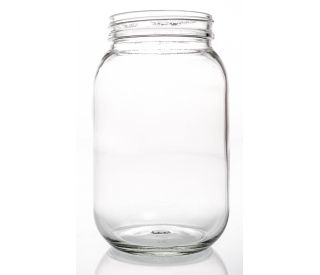
\includegraphics[width=0.3\textwidth,height=0.2\textheight]{GlassCup}}
	\subcaptionbox{SS bottle \label{StainlessSteel} [\citenum{PeaceWithTheWildLimited}]}
	{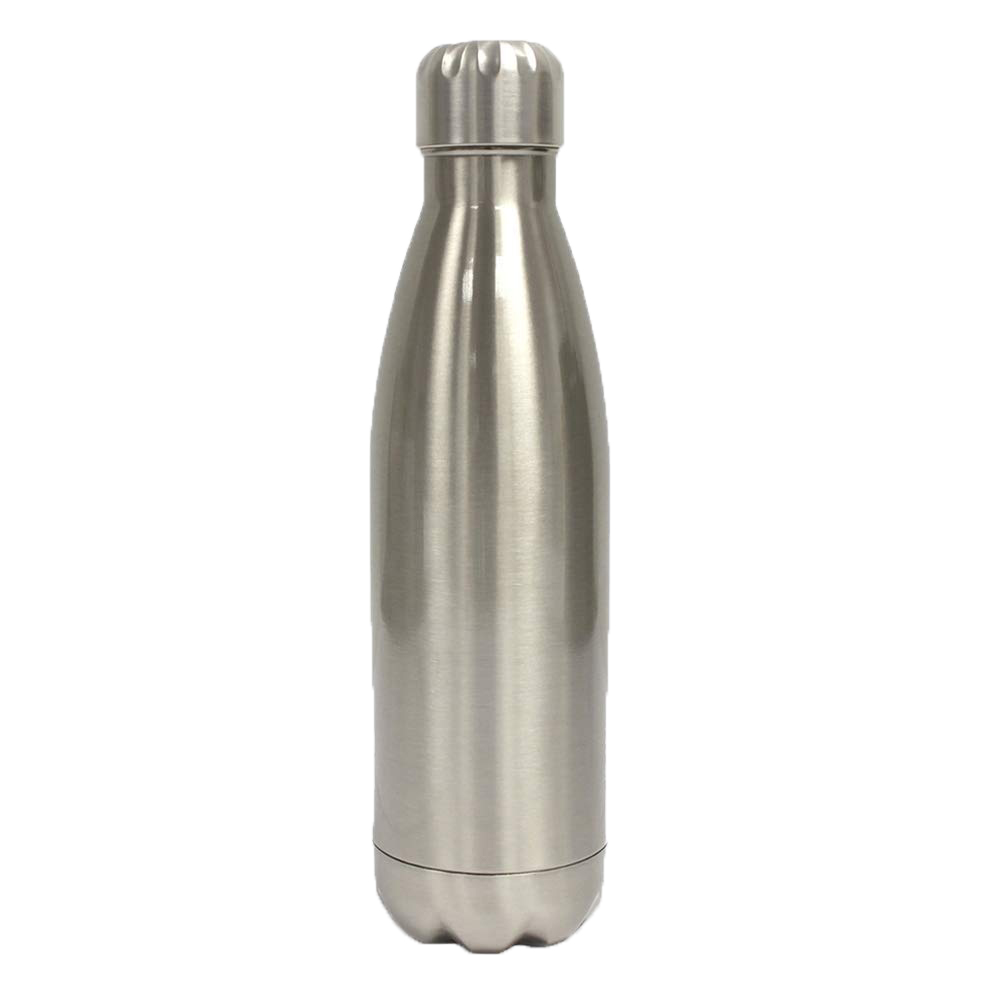
\includegraphics[width=0.3\textwidth,height=0.16\textheight]{StainlessSteel}}
	\subcaptionbox{Thermos bottle \label{Thermos} [\citenum{ThermosL.L.C.}]}
	{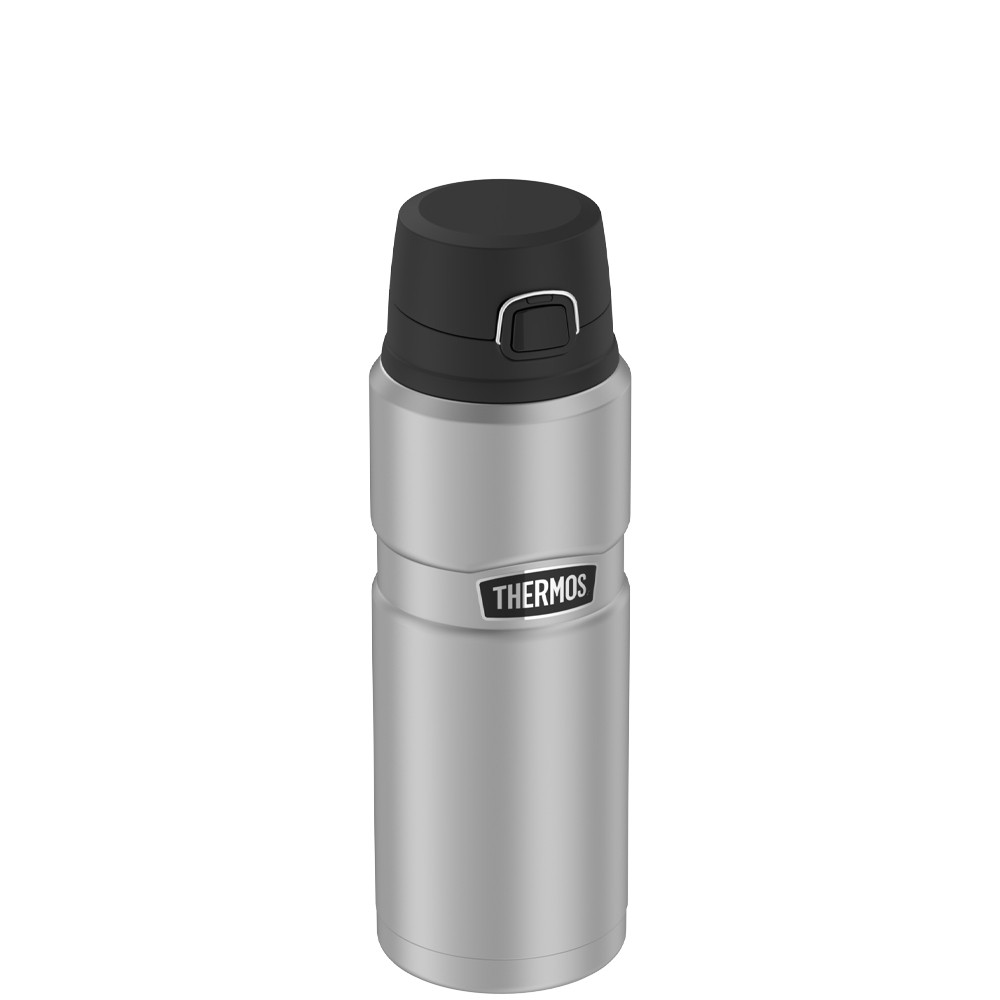
\includegraphics[width=0.3\textwidth,height=0.2\textheight]{Thermos}}
	\caption{Different types of containers with lids were used for testing. (PS = Polystyrene, PP = Polypropylene, SS = Stainless Steel). They were all rinsed with clean water and left to dry at the room temperature (20 °C) before the experiment was implemented. }
	\label{Figure 3}
\end{figure}

\pagebreak

\subsection*{Procedure}

The experiment was conducted at room temperature (20 °C) for over eight hours. Hot water was added into the coffee until the substance achieved a temperature of 70°C. One of the two thermos flasks was rinsed with hot water at a temperature of 70°C before the experiment proceeded. After that, the coffee was divided into equal portions, which were poured into the containers using a measuring cup. The containers were closed immediately to prevent heat loss and stored in a dark, moderately cool place. Every hour, the temperature of the content inside each container was measured one at a time. 
%----------------------------------------------------------
\section*{Results}

\subsection*{Part 1}

\begin{figure}[h!]
\centering
\resizebox{0.9\textwidth}{0.5\textheight}
{
	\begin{tikzpicture}
		\begin{axis}[
			xlabel = Hour,
			ylabel = Temperature (°C),
			transpose legend,
			legend columns=-1,
			legend style={at={(0.5,1.05)},anchor=south},
			]
			\addplot
			table[x=a,y=b,col sep=comma] {data.csv};
			\addplot
			table[x=a,y=c,col sep=comma] {data.csv}; 
			\addplot
			table[x=a,y=d,col sep=comma] {data.csv};
			\addplot
			table[x=a,y=e,col sep=comma] {data.csv};
			\addplot
			table[x=a,y=c,col sep=comma] {data.csv};
			\legend{Thermos,Glass,Polypropylene,Stainless Steel, Styrofoam}
		\end{axis}
	\end{tikzpicture}
}
	\caption{Temperature of coffee in five containers over eight hours. All specimen were not rinsed with hot water in this part of the experiment.}
	\label{Figure 4}
\end{figure}


Most containers fail to retain the ideal temperature region for the coffee for a long duration. While other containers all reach the room temperature after approximately 5 hours, coffee in the Thermos only reduces slightly over 8 hours from 67.4 ℃ to 62  ℃ (as seen in \autoref{Figure 2}). There was also a variation in the heat loss rates. A steep decrease in the internal temperature was recorded in the bottle made of stainless steel, from 68.6 ℃ to 25.4  ℃ in just an hour (\autoref{Figure 2}). Compared to the Thermos and PS containers’, glass and polypropylene lines express a non-linear pattern like the Stainless-steel line (\autoref{Figure 2}). 

\subsection*{Part 2}

\begin{table}[h!]
	\centering
	\begin{threeparttable}
		\caption{Mean (M) and standard deviation (SD) of the coffee temperature (in degree Celsius) in two types of thermos used in the experiment. A p-value and a t-value from the two-tailed t-distribution test are also included.}
		\label{Table 2}
		\begin{tabular*}{\textwidth}{ @{\extracolsep{\fill}} ccccc}
			\toprule
			Type & M & SD & p-value & t–value (two tails)\\
			\midrule 
			Unrinsed 		& 64.91   &1.89		&						&		 \\
						&		  &		    &1.47$\times10^{-7}$ 	&-3.54	 \\			
			Rinsed  	& 68.00   &1.58	&							&	 	 \\
			\bottomrule
		\end{tabular*}
%		\begin{tablenotes}
%			\footnotesize
%			\centering
%			\item Note: M is mean; SD is standard deviation
%		\end{tablenotes}
	\end{threeparttable}
\end{table}

The proposed hypothesis was assessed in this part. As seen in \autoref{Table 2}, the temperature of coffee in the unrinsed vacuum flask over eight hours (M = 64.91; SD = 1.89) was lower than its unrinsed counterpart (M = 68.00; SD = 1.58). Furthermore, the results from the Two-sample t-test (\autoref{Table 2}, p = 1.47$\times10^{-7} < $ 0.05) consolidates that hot water rinsing does improve the heat preservation effects of the thermos.
%-------------------------------------------------------------------------
\section*{Discussion}

According to \autoref{Figure 4}, it is apparent that the thermos bottle was the only one that fulfilled the criteria required for an ideal coffee container. The rinsed (M = 68.00; SD = 1.58, \autoref{Table 2}) and unrinsed (M = 64.91; SD = 1.89, \autoref{Table 2}) vacuum containers managed to keep the temperature in the favourable range (\SI{52}{\celsius} – \SI{68}{\celsius}) even after eight hours. All other containers failed to retain the required temperature for a perfect cup of coffee after just one hour, except for the Styrofoam cup which was at 55.1 ℃ (\autoref{Figure 2}). Hence, Styrofoam cups can be a short-term alternative to thermos flasks for storing newly brewed coffee. Stainless steel, glass and Polypropylene bottles are not practical for hot beverages due to their high thermal transfer rate. It did not only lead to a steady drop in the drink’s temperature but also a scorching outer case because of the absorbed heat in the short term. Accordingly, attention to the choice of material is required when drinkers need to store hot beverages.

The thermos flask properties are contributed to its design. It has a container with a double wall with the air inside removed to create a vacuum. The heat transfer between the content and the environment almost mitigates as the vacuum is one of the best insulators as seen in \autoref{Table 1}. Another factor is the silver coating of the inner chamber. \citeauthor{Liu2020} suggested that polylactic acid (PLA) films with silver nanoparticles (AgNPs) contributed to an improvement in the thermal insulation of Nickel-Titanium Alloy. However, this ability can still be enhanced as proven in the results ($M_{rinsed} = 68.00 > M_{unrinsed}$ = 64.91, \autoref{Table 2}). A likely explanation is that the cold interior of the container can absorb external heat from the coffee. Thus, it is recommended for consumers to rinse their thermos flask with hot water before storing coffee for the best result.

This study is one of the only few to investigate the influences of containers on the drink temperature. One research \citep{Bailey2008} investigated the thermal performance of aluminium and glass beer bottles using a computational simulation. In contrary to our findings, their paper suggested that thermal conductivity of bottles' material has negligible importance on the content. The contrary highlights some limitations of this research. Due to the technically oriented nature of the questions, more specialised tools are compulsory for the accuracy of the results. Another aspect is that heat does not only transfer by conduction but also through radiation and convection. Although there is no heat conduction in space, radiation from the electromagnetic waves enables thermal exchange in a vacuum. It is a variable that the research did not take into account but will address in the future.

%---------------------------------------------------------------------------------------
\section*{Conclusions}

Coffee has become an integral part of the daily lives of many people. The paper will be of interest to consumers who wish to enjoy freshly brewed coffee even after an extended duration. Before this study, there was a lack of insights into the insulation capabilities of beverage canisters. By comparing the temperature of the freshly brewed coffee in drink containers over eight hours, the study validates that thermos flask is indeed the best choice for consumers. It managed to keep the drink at the ideal temperature for the longest time. While not as potent as the thermos flasks, Styrofoam cup is indicated to be suitable for short-term consumption as the coffee in it is still hot enough after an hour. Stainless steel, polypropylene and glass bottle demonstrated a lack of insulation leading to drastic drops in the liquid temperature. On the other hand, empirical data from the Two-sample t-test shown that hot rinsing improved the heat insulation in beverage containers. Overall, the research further reinforces the correlation between the thermal conductivity and heat transfer process.
 
%----------------------------------------------------------------------------------
	\bibliography{library}
%-----------------------------------------------------------------------------------------
\end{document}          
